\section{Diffusion Language Models}

\begin{frame}{}
    \LARGE Research Frontiers: \textbf{Diffusion Language Models}

    \vspace{1em}
    \normalsize Must text be generated one token at a time?
\end{frame}

\begin{frame}{Five Open Problems of 2025, and Who Closed Them}
    \begin{itemize}\itemsep0.3em
        \item LLaDA (2025) scaled masked diffusion to 8B parameters and left five problems open. This section follows each one.
    \end{itemize}
    \begin{center}
    \small
    \renewcommand{\arraystretch}{1.25}
    \setlength{\tabcolsep}{4pt}\begin{adjustbox}{max width=\linewidth}\begin{tabular}{lll}
        \toprule
        \textbf{Open problem in 2025} & \textbf{Status, Oct 2026} & \textbf{What addressed it} \\
        \midrule
        Answer length fixed in advance & largely solved & block diffusion, in all 2026 products \\
        No KV cache & solved in part & approximate caches, exact for finished blocks \\
        No RL or preference alignment & \alert{superseded} & d1, LLaDA 1.5, large-scale RL in LLaDA2.1 \\
        Likelihood is a Monte Carlo bound & still open & now the bottleneck for RL \\
        Comparison with AR not controlled & partly & controlled studies exist. AR is still ahead \\
        \bottomrule
    \end{tabular}\end{adjustbox}
    \end{center}
    \src{Problems: Nie et al., ``Large Language Diffusion Models,'' NeurIPS 2025, \href{https://arxiv.org/abs/2502.09992}{arXiv:2502.09992}. Status: \href{https://arxiv.org/abs/2503.09573}{arXiv:2503.09573}, \href{https://arxiv.org/abs/2505.22618}{arXiv:2505.22618}, \href{https://arxiv.org/abs/2504.12216}{arXiv:2504.12216}, \href{https://arxiv.org/abs/2602.08676}{arXiv:2602.08676}, \href{https://arxiv.org/abs/2606.19475}{arXiv:2606.19475}.}
\end{frame}

\begin{frame}{The Theory: Masked Diffusion Is Weighted Masked LM}
    \begin{itemize}\itemsep0.35em
        \item \textbf{D3PM (2021)} defined diffusion on discrete tokens. Its \emph{absorbing} variant sends tokens to a mask state.
        \item \textbf{MDLM and MD4 (2024)} showed that the continuous-time training bound is simply
        \[
            \mathcal{L}^{\infty}_{\text{NELBO}} = \mathbb{E}_q \int_{0}^{1} \frac{\alpha'_t}{1-\alpha_t}\,\log\big\langle \mathbf{x}_\theta(\mathbf{z}_t,t),\,\mathbf{x}\big\rangle\,dt
        \]
        a \emph{weighted mixture of masked-language-modelling losses}. BERT with a random mask rate.
        \item \textbf{The likelihood gap is real at small scale.} Perplexity on LM1B after 33B training tokens: autoregressive 22.32, MDLM at most 27.04, the earlier SEDD at most 32.79. After 327B: 20.86 against at most 23.00. A 2026 controlled study still finds GPT-2 at 20.98 against MDLM at 28.45 on OpenWebText.
        \item \textbf{Noise is a design choice.} Masking trains faster. Uniform noise lets any token be revised later.
    \end{itemize}
    \src{Austin et al., \href{https://arxiv.org/abs/2107.03006}{arXiv:2107.03006}. Sahoo et al., ``MDLM,'' \href{https://arxiv.org/abs/2406.07524}{arXiv:2406.07524}, Eq. 12 and Table 1. Shi et al., ``MD4,'' \href{https://arxiv.org/abs/2406.04329}{arXiv:2406.04329}. Bertolani et al., \href{https://arxiv.org/abs/2606.19475}{arXiv:2606.19475}. Kuleshov, ``How to Build a Diffusion Language Model'' (2026).}
\end{frame}

\begin{frame}{Block Diffusion: Autoregressive Between Blocks, Diffusion Inside}
    \[
        \log p_\theta(\mathbf{x}) = \sum_{b=1}^{B}\log p_\theta\big(\mathbf{x}^b\mid\mathbf{x}^{<b}\big), \qquad \text{each block conditional is a masked diffusion}
    \]
    \begin{center}
    \begin{adjustbox}{max width=\linewidth}\begin{tikzpicture}[font=\scriptsize, >=Stealth]
        \draw[fill=gray!25] (0,0) rectangle (2.2,0.6);
        \node at (1.1,0.3) {prompt};
        \draw[fill=KAUSTcyan!30] (2.4,0) rectangle (4.6,0.6);
        \node at (3.5,0.3) {block 1, clean};
        \draw[fill=KAUSTcyan!30] (4.8,0) rectangle (7.0,0.6);
        \node at (5.9,0.3) {block 2, clean};
        \draw[fill=darkorange!35, thick] (7.2,0) rectangle (9.4,0.6);
        \node at (8.3,0.3) {block 3, noised};
        \draw[dashed] (9.6,0) rectangle (11.8,0.6);
        \node[gray] at (10.7,0.3) {block 4};
        \draw[thick, KAUSTblue] (0,-0.15) -- (0,-0.3) -- (7.0,-0.3) -- (7.0,-0.15);
        \node[KAUSTblue] at (3.5,-0.55) {causal context, exact KV cache};
        \draw[thick, darkorange!80!black] (7.2,-0.15) -- (7.2,-0.3) -- (9.4,-0.3) -- (9.4,-0.15);
        \node[darkorange!80!black] at (8.3,-0.55) {bidirectional denoising};
    \end{tikzpicture}\end{adjustbox}
    \end{center}
    \begin{itemize}\itemsep0.4em
        \item A block of 1 token is autoregression. A block of the whole sequence is LLaDA.
        \item It gives \textbf{any output length} and \textbf{exact KV caching} of finished blocks.
        \item 2026 systems use blocks of 32 tokens up to a 256-token canvas (DiffusionGemma).
        \item \textbf{The price:} left-to-right order returns between blocks.
    \end{itemize}
    \src{Arriola et al., ``Block Diffusion: Interpolating Between Autoregressive and Diffusion Language Models,'' \href{https://arxiv.org/abs/2503.09573}{arXiv:2503.09573}. Bie et al., \href{https://arxiv.org/abs/2512.15745}{arXiv:2512.15745}. DiffusionGemma model card (June 2026).}
\end{frame}

\begin{frame}{The 2025 to 2026 Landscape: Converted, Not Trained from Scratch}
    \begin{center}
    \footnotesize
    \renewcommand{\arraystretch}{1.04}
    \begin{adjustbox}{max width=\linewidth}\begin{tabular}{llll}
        \toprule
        \textbf{Model (date)} & \textbf{Size} & \textbf{Starting point} & \textbf{Reported speed} \\
        \midrule
        Dream 7B (Aug 2025) & 7B & Qwen2.5 7B weights & not the focus \\
        Gemini Diffusion (experimental) & not disclosed & not disclosed & 1,479 tok/s \\
        LLaDA2.1 (Feb 2026) & 16B and 100B MoE & AR models & 892 tok/s (HumanEval+) \\
        Mercury 2 (2026, closed) & not disclosed & not disclosed & about 1,000 tok/s (vendor) \\
        Nemotron-Labs (May 2026) & 3B, 8B, 14B & AR pre-training & about 865 tok/s (B200) \\
        \rowcolor{KAUSTcyan!12} DiffusionGemma (Jun 2026) & 25.2B, 3.8B active & Gemma 4 26B-A4B & over 1,100 tok/s (H100) \\
        \bottomrule
    \end{tabular}\end{adjustbox}
    \end{center}
    \begin{itemize}\itemsep0.4em
        \item \textbf{Conversion is the default.} LLaDA2.0 grows the block size from 1 token to the full sequence, trains there, then shrinks it back to small blocks.
        \item \textbf{One network, three modes.} Nemotron-Labs decodes autoregressively, by diffusion, or drafts a block and verifies it causally in the same model.
        \item \textbf{``Fastest'' claims are not comparable.} Hardware, batch and measurement differ across vendors.
    \end{itemize}
    \src{Ye et al., \href{https://arxiv.org/abs/2508.15487}{arXiv:2508.15487}. Google DeepMind, Gemini Diffusion page and DiffusionGemma card. Bie et al., \href{https://arxiv.org/abs/2512.15745}{arXiv:2512.15745}, \href{https://arxiv.org/abs/2602.08676}{arXiv:2602.08676}. Inception Labs, Mercury 2 blog. NVIDIA, Nemotron-Labs Diffusion blog (May 2026).}
\end{frame}

\begin{frame}{The Honest Comparison: Same Family, Same Data}
    \begin{columns}[T,onlytextwidth]
        \column{0.5\textwidth}
        \centering
        \begin{adjustbox}{max width=\linewidth}\begin{tikzpicture}
            \begin{axis}[ybar, width=7.0cm, height=5.3cm, bar width=0.24cm,
                ymin=0, ymax=100, ylabel={\scriptsize score},
                symbolic x coords={A,B,C,D,E}, xtick=data,
                xticklabels={MMLU-Pro, GPQA-D, LiveCodeBench v6, AIME 2026, BBEH},
                x tick label style={font=\tiny, rotate=20, anchor=east},
                y tick label style={font=\scriptsize},
                legend style={font=\tiny, at={(0.5,1.03)}, anchor=south, legend columns=2, draw=none},
                axis lines=left, enlarge x limits=0.13]
                \addplot[fill=gray!45, draw=gray!70!black] coordinates {(A,82.6) (B,82.3) (C,77.1) (D,88.3) (E,64.8)};
                \addplot[fill=darkorange!65, draw=darkorange!80!black] coordinates {(A,77.6) (B,73.2) (C,69.1) (D,69.1) (E,47.6)};
                \legend{Gemma 4 26B-A4B (autoregressive), DiffusionGemma}
            \end{axis}
        \end{tikzpicture}\end{adjustbox}
        \column{0.48\textwidth}
        \begin{itemize}\itemsep0.45em
            \item DiffusionGemma is built \emph{on} Gemma 4 26B-A4B. It loses \alert{5 to 19 points}, most on hard reasoning.
            \item \textbf{Where diffusion wins:} global constraints. Dream 7B solves Sudoku at 81.0\%, against 21.0\% for the Qwen2.5 it started from.
            \item A 2026 controlled study: \emph{``No single diffusion paradigm dominates.''}
        \end{itemize}
    \end{columns}
    \vspace{0.2em}
    \takeaway{Today's trade: roughly 2x to 4x speed for real reasoning points.}
    \src{Google, DiffusionGemma model card (updated 2026-06-10). Ye et al., ``Dream 7B,'' \href{https://arxiv.org/abs/2508.15487}{arXiv:2508.15487}. Bertolani et al., ``Diffusion Language Models: An Experimental Analysis,'' \href{https://arxiv.org/abs/2606.19475}{arXiv:2606.19475}.}
\end{frame}

\begin{frame}{Making It Fast: Caches and Confident Parallel Unmasking}
    \centering
    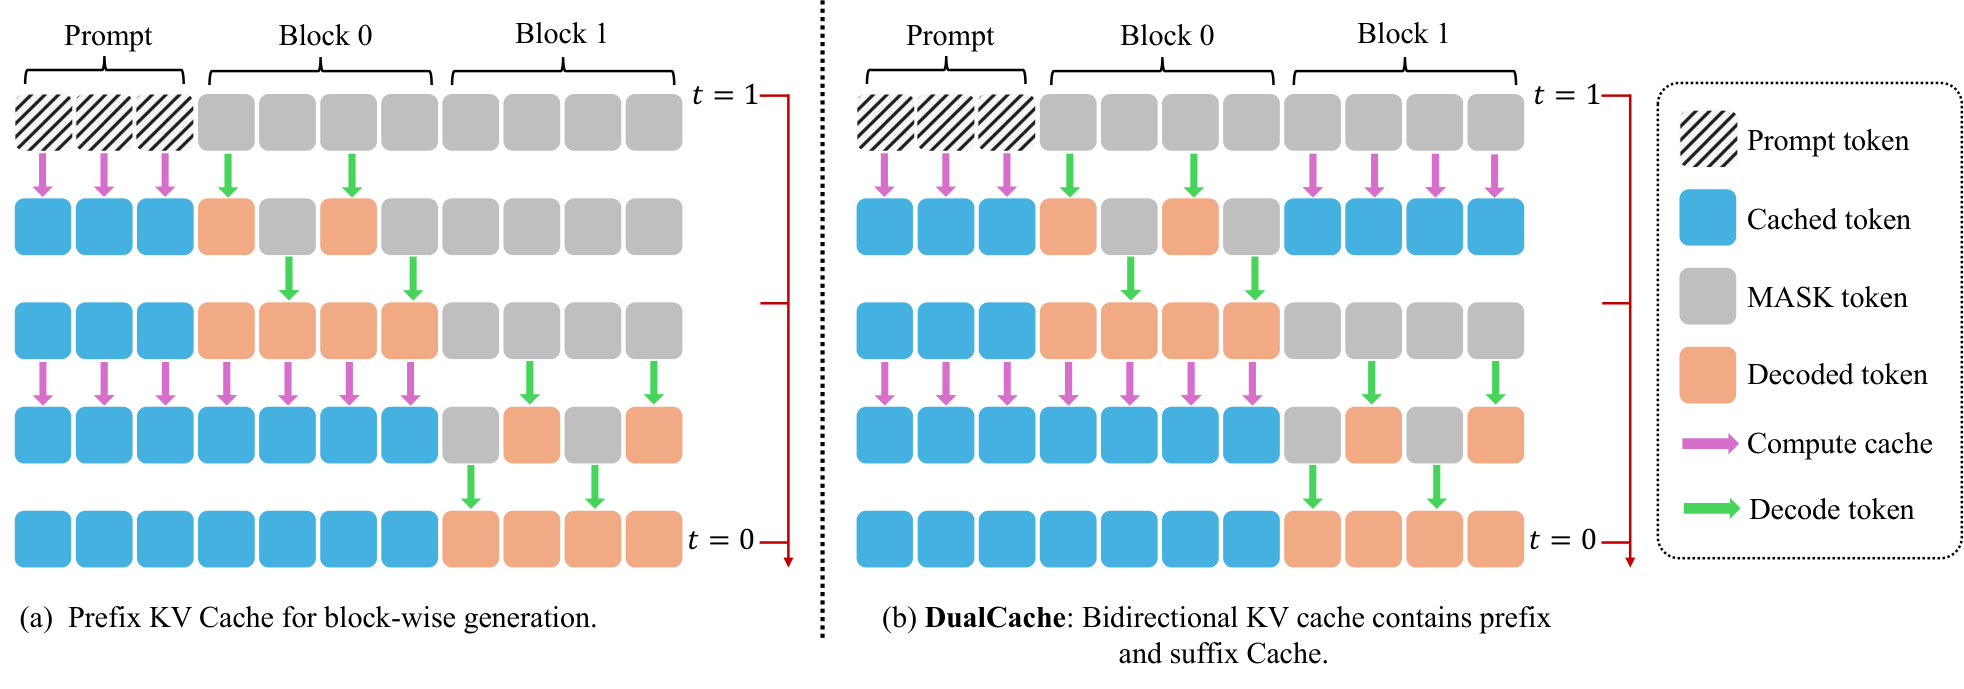
\includegraphics[width=0.9\linewidth,height=0.36\textheight,keepaspectratio]{images/research-frontiers/fastdllm_kvcache.png}
    \begin{itemize}\itemsep0.3em
        \item \textbf{Cache.} Between denoising steps most activations barely change, so reuse KV for the prefix and for the masked suffix.
        \item \textbf{Unmask in parallel, but only when sure.} Tokens above a confidence threshold (default 0.9) are committed together. The analogue of acceptance in speculative decoding.
        \item \textbf{Read the baseline.} LLaDA on GSM8K goes from 6.7 to 54.4 tokens/s (8.1x) at nearly the same accuracy. Against an \emph{autoregressive} model the gains are 2.1x (LLaDA2.0) and 2.5x (Fast-dLLM v2).
    \end{itemize}
    \src{Wu et al., ``Fast-dLLM,'' \href{https://arxiv.org/abs/2505.22618}{arXiv:2505.22618}, cache figure and Table 1. Wu et al., ``Fast-dLLM v2,'' \href{https://arxiv.org/abs/2509.26328}{arXiv:2509.26328}. Bie et al., ``LLaDA2.0,'' \href{https://arxiv.org/abs/2512.15745}{arXiv:2512.15745}.}
\end{frame}

\begin{frame}{RL for Diffusion LMs: the Likelihood Problem}
    \begin{itemize}\itemsep0.35em
        \item Policy-gradient methods such as GRPO need $\log \pi_\theta(\text{output})$. A diffusion LM has no cheap exact token likelihood.
        \item \textbf{d1 (2025)} estimates it in \emph{one unmasking step} with a mean-field sum $\sum_k \log\pi_\theta(o^k\mid q)$, and runs a GRPO-style update (diffu-GRPO).
    \end{itemize}
    \begin{center}
    \small
    \begin{adjustbox}{max width=\linewidth}\begin{tabular}{lcccc}
        \toprule
        \textbf{LLaDA-8B-Instruct, length 256} & \textbf{GSM8K} & \textbf{MATH500} & \textbf{Countdown} & \textbf{Sudoku} \\
        \midrule
        Base model & 76.7 & 32.4 & 19.5 & 6.7 \\
        + diffu-GRPO & 79.8 & 37.2 & 31.3 & 12.9 \\
        \rowcolor{KAUSTcyan!12} d1 (SFT, then diffu-GRPO) & 81.1 & 38.6 & 32.0 & 16.7 \\
        \bottomrule
    \end{tabular}\end{adjustbox}
    \end{center}
    \begin{itemize}\itemsep0.35em
        \item Later estimators lower the variance (LLaDA 1.5) or score the whole sequence (ESPO).
    \end{itemize}
    \takeaway{RL for diffusion now runs at scale in LLaDA2.1. Every method still leans on a biased or high-variance likelihood surrogate.}
    \src{Zhao, Gupta, Zheng, Grover, ``d1: Scaling Reasoning in Diffusion LLMs via RL,'' \href{https://arxiv.org/abs/2504.12216}{arXiv:2504.12216}, Table 1. Zhu et al., \href{https://arxiv.org/abs/2505.19223}{arXiv:2505.19223}. Ou et al., ``ESPO,'' \href{https://arxiv.org/abs/2512.03759}{arXiv:2512.03759}. Bie et al., \href{https://arxiv.org/abs/2602.08676}{arXiv:2602.08676}.}
\end{frame}

\begin{frame}{A Live Debate: Is Diffusion More Data-Efficient?}
    \begin{center}
    \small
    \renewcommand{\arraystretch}{1.2}
    \begin{adjustbox}{max width=\linewidth}\begin{tabular}{>{\raggedright\arraybackslash}p{4.3cm}>{\raggedright\arraybackslash}p{8.9cm}}
        \toprule
        \textbf{Position} & \textbf{Evidence} \\
        \midrule
        \textbf{Yes, when data is scarce} (CMU, 2025) & repeated data stays useful for about 100 epochs, against about 4 for AR \\
        \textbf{Yes, sooner for larger models} (Ni et al., 2025) & a 1.7B diffusion coder on 10B unique tokens beats a matched AR coder \\
        \textbf{Only if over-parameterised} (ETH, 2025) & with early stopping, AR is better at every width \\
        \textbf{No, under a compute limit} (survey, 2026) & \emph{``substantially more data-hungry under compute constraints''} \\
        \bottomrule
    \end{tabular}\end{adjustbox}
    \end{center}
    \begin{itemize}\itemsep0.4em

        \item The accurate statement: \textbf{diffusion trades compute for data}. Each source attaches a regime.
        \item No independent replication above 2B parameters was found.
    \end{itemize}
    \src{Prabhudesai et al., ``Diffusion Beats Autoregressive in Data-Constrained Settings,'' \href{https://arxiv.org/abs/2507.15857}{arXiv:2507.15857}. Ni et al., \href{https://arxiv.org/abs/2511.03276}{arXiv:2511.03276}. Fraij, Dauncey, \href{https://arxiv.org/abs/2509.24974}{arXiv:2509.24974}. Li, Chen, Guo, Shen, \href{https://arxiv.org/abs/2508.10875}{arXiv:2508.10875}.}
\end{frame}

\begin{frame}{Diffusion LMs: What to Remember}
    \begin{itemize}\itemsep0.55em
        \item Masked diffusion is \textbf{masked language modelling with a weighted, random mask rate}.
        \item The 2026 systems are \textbf{converted from autoregressive models} and decode \textbf{block by block}.
        \item Speed is real: about \textbf{2x over autoregressive serving}. The 8x figures are against slow diffusion baselines.
        \item Quality is not free: \textbf{5 to 19 points} below the autoregressive sibling, with wins on globally constrained tasks.
        \item Open: RL without exact likelihoods, serving at high batch, and whether speed is the \emph{only} advantage.
    \end{itemize}
    \vspace{0.4em}
    \takeaway{\textbf{Next.} So far we moved and compressed \emph{computation}. The other thing a model holds is \emph{knowledge}. Where is it stored, and can it be updated?}
\end{frame}
